\documentclass[a4paper,10pt]{article}
\usepackage[utf8]{inputenc}

\usepackage[english]{babel}
\usepackage[dvinames]{xcolor}
\usepackage[compact,small]{titlesec}
\usepackage{booktabs}
\usepackage{multirow}
\usepackage{amsfonts,amsmath,amssymb}
\usepackage{marginnote}
\usepackage[top=1.8cm, bottom=1.8cm, outer=1.8cm, inner=1.8cm, heightrounded, marginparwidth=2.5cm, marginparsep=0.5cm]{geometry}
\usepackage{enumitem}
\setlist{noitemsep,parsep=2pt}
\newcommand{\highlight}[1]{\textcolor{kuleuven}{#1}}
%\usepackage{pythonhighlight}
\usepackage{cleveref}
\usepackage{graphicx}
%\usepackage{subfigure}
\usepackage{float}
\usepackage{caption}
\usepackage{subcaption}


\newcommand{\nextyear}{\advance\year by 1 \the\year\advance\year by -1}
\newcommand{\thisyear}{\the\year}
\newcommand{\deadlineGroup}{November 27, \thisyear{} at 16:00 CET}
\newcommand{\deadlineCode}{December 18, \thisyear{} at 16:00 CET}
\newcommand{\deadlineReport}{January 4, \nextyear{} at 16:00 CET}

\newcommand{\ReplaceMe}[1]{{\color{blue}#1}}
\newcommand{\RemoveMe}[1]{{\color{purple}#1}}

\setlength{\parskip}{5pt}

%opening
\title{Evolutionary Algorithms: Final report}
\author{Georgios Kouros (r0816917)}

\begin{document}
\fontfamily{ppl}
\selectfont{}

\maketitle

\section{Metadata}

\begin{itemize}
 \item \textbf{Group members during group phase:} Kostantinos Gkentsidis and Jeffrey Quicken
 \item \textbf{Time spent on group phase:} 15 hours
 \item \textbf{Time spent on final code:} 45 hours
 \item \textbf{Time spent on final report:} 12 hours
\end{itemize}

\section{Modifications since the group phase}

%\RemoveMe{\textbf{Goal:} Based on this section, we will evaluate insofar as you are able to analyse common problems arising in the design and implementation of evolutionary algorithms and your ability to effectively solve them.}

\subsection{Main improvements}

%\ReplaceMe{List the main changes that you implemented since the group phase. You do not need to explain the employed techniques in detail; for this, you should refer to the appropriate subsection of section 3 of the report.}

%\paragraph{} \ReplaceMe{Short description 1: State what modification you made (e.g., replaced top-$\lambda$ selection with $k$-tournament selection). What aspect of your evolutionary algorithm did it improve?} 

\paragraph{Greedy Heuristic Initialization}: Added a heuristic initialization of candidate solutions in order to inject some good initial candidates to the random initial population and speed up the search of the optimum. For more information see Subsection \ref{ss:initialization}.

\paragraph{Local Search:} Converted the evolutionary algorithm to a memetic algorithm through the inclusion of 2-opt local search after the variation step of each iteration. This addition significantly improved convergence to really good candidate solutions. For more information see Subsection \ref{ss:local_search}.

%\paragraph{Mutation Self-Adaptivity:} Self-adaptivity was added to vary mutation rate and strength in order to improve the diversity of the population across iterations and prevent premature convergence.

\paragraph{Diversity Promotion}: Fitness sharing was added to the $(\lambda+\mu)$~elimination step to improve the diversity of the population across iterations and prevent premature convergence. For more information see Subsections \ref{ss:elimination} and \ref{ss:diversity_promotion} .

\paragraph{Greedy Mutation:} Added a new mutation operator that uses a greedy approach to adapt an individual in the optimal way. For more information see Subsection \ref{ss:mut}


\subsection{Issues resolved}
%\ReplaceMe{Recall the list of issues from the group phase. Describe how you solved these issues in the individual phase.}

%\paragraph{}\ReplaceMe{Short description 1: Describe the observation or problem from the group phase. Explain what caused this issue. How did you solve it (you can refer to the list of improvements)? Did fixing it significantly benefit your evolutionary algorithm? If you did not fix it: why not?}

\paragraph{Depleting Diversity:} In the group phase, we detected a problem with diversity, meaning that our algorithm converged prematurely to locally optimal candidate solutions, thus preventing the discovery of better solutions. This issue was fixed through the addition of diversity promotion, increased mutation strength, and varying mutation operators.

\paragraph{Premature convergence:} In the group phase, we used the $(\lambda+\mu)-elimination$ in combination with a convergence criterion of matching mean to best fitness. This resulted in a mostly exploitative behavior resulting in premature convergence. This issue was fixed by implementing methods for diversity promotion.

\paragraph{Loss of Best Candidate:} In the individual phase it was discovered that sometimes the best candidate was lost across iterations. This was easily visible as unexplained spikes in the corresponding graph across iterations. This happened due to an unwanted modification of the original population during mutation. Fixing this bug cleared this error.

\paragraph{Inefficient Crossover Operator:} The code used for the Order Crossover operator was taken from stackoverflow. In an effort to refine this code and remove needless code repetition, the operator was rewritten from scratch and ended up being more efficient, shorter and more readable.

\section{Final design of the evolutionary algorithm} 

%\RemoveMe{\textbf{Goal:} Based on this section, we will evaluate insofar as you are able to design and implement an advanced, effective evolutionary algorithm for solving a model problem.}

%\ReplaceMe{In this section, you should describe all components of your final evolutionary algorithm and how they fit together.}

\subsection{Representation} \label{ss:representation}

%\ReplaceMe{How do you represent the candidate solutions? What is your motivation to choose this one? What other options did you consider? How did you implement this specifically in Python (e.g., a list, set, numpy array, etc)?}

In Davis et al ~\cite{davis}, five different representations are presented for TSP: Binary, Path, Adjacency, Ordinal, and Matrix representations. Based on a review of the different methods in the same research, it was decided in the group phase to select the \textbf{Path} / \textbf{Permutation Representation}, because of its better performance, operator variety, and explainability. The same representation was kept in the individual phase. This  Path representation was implemented as a python class called Individual that stores a list of integers representing indices of cities with respect to the given distance matrix. The route of the candidate solution is checked against errors on update and hence the use of python sets was deemed redundant.

\subsection{Initialization} \label{ss:initialization}

%\ReplaceMe{How do you initialize the population? How did you determine the number of individuals? Did you implement advanced initialization mechanisms (local search operators, heuristic solutions)? If so, describe them. Do you believe your approach maintains sufficient diversity? How do you ensure that your population enrichment scheme does not immediately take over the population? Did you implement other initialization schemes that did not make it to the final version? Why did you discard them? How did you determine the population size?}

In the group phase, a random initialization was used for the population resulting in high diversity with a high probability given a big enough population size $\lambda$. In order to achieve good results, it was decided to use a quite large population (1000-2000).

In the individual phase, the initialization step was augmented with a number of greedy heuristic candidate solutions in order to provide some direction to the search and avoid reinventing the wheel. The greedy heuristic search starts from a random city keeps following the shortest path from city to city until all cities are visited exactly once and finally ends up on the first city.  

The use of really good candidate solutions entails the danger of taking over the population fairly quickly. However, this issue can be mitigated by limiting the number of heuristic candidate solutions or limiting the steps of the greedy search. Both methods were implemented and based on experiments it was decided to apply greedy search for $10\%$ of the initial population

Furthermore, the addition local search and diversity promotion, allowed the use of a population and offspring size that's two magnitudes smaller ($\lambda = 10, \mu=5$). Using a lower population and offspring size resulted in better performance with more iterations and no impact on the final results.

\subsection{Selection operators} \label{ss:selection}

%\ReplaceMe{Which selection operators did you implement? If they are not from the slides, describe them. Can you motivate why you chose this one? Are there parameters that need to be chosen? Did you use an advanced scheme to vary these parameters throughout the iterations? Did you try other selection operators not included in the final version? Why did you discard them?}
Similarly to the group phase, \textit{k-tournament selection} was picked for the individual phase as well. This selection method performed really well before and offered a nice balance between exploration and exploitation, hence it was kept in this phase as well. The only tunable parameter of this selection operator is the number $k$ of individuals that take part in a tournament.

\subsection{Mutation operators} \label{ss:mut}

%\ReplaceMe{Which mutation operators did you implement? If they are not from the slides, describe them. How do you choose among several mutation operators? Do you believe it will introduce sufficient randomness? Can that be controlled with parameters? Do you use self-adaptivity? Do you use any other advanced parameter control mechanisms (e.g., variable across iterations)? Did you try other mutation operators not included in the final version? Why did you discard them?}

In the group phase, two mutation methods were used, namely inversion mutation and swap mutation. Both mutation operators, were extended in the individual phase with a new parameter called mutation strength $\sigma_\mu$, which determines the number of successive applications of the operator on an individual.

Besides, those two mutation operators, a new greedy mutation operator was implemented in the individual phase. This operator removes four edges from a route randomly, resulting in five unconnected segments, which are greedily reconnected by finding the segment permutation with the best fitness.

Initially each mutation operator was assigned equal probability $33.333\%$ to be chosen. However, in a trial of adaptive parameter control with a reward system, it was discovered that the greedy mutation operator improved solutions more consistently and took over the operator selection, so in the end it was decided to use only the greedy mutation operator.

\subsection{Recombination operators} \label{ss:recombination}

%\ReplaceMe{Which recombination operators did you implement? If they are not from the slides, describe them. How do you choose among several recombination operators? Why did you choose these ones specifically? Explain how you believe that these operators can produce offspring that combine the best features from their parents. How does your operator behave if there is little overlap between the parents? Can your recombination be controlled with parameters; what behavior do they change? Do you use self-adaptivity? Do you use any other advanced parameter control mechanisms (e.g., variable across iterations)? Did you try other recombination operators not included in the final version? Why did you discard them? Did you consider recombination with arity strictly greater than 2?}

In the individual phase, it was decided to reuse the \textit{Order Crossover} \cite{davis} operator, since it performs really well for order-based permutation problems like TSP according to the literature eg. \cite{memetic} and based on experiments. The only change regarding this operator was the rewritting of its code to make it more efficient and readable.

The operator consists of the following steps:
\begin{enumerate}
\item Copy a segment between two randomly generated crossover points of the first parent to the first child.
\item Starting from the second crossover point on the second parent this time, start copying its genes/alleles that are not already contained on the child, until the child is full.
\item Create the second child like the first but with the reverse order of the parents.
\end{enumerate}

One advantage of this operator is that it ensures the generation of only valid offspring and thus doesn't require the need to implement a repair mechanism. Moreover, the fact that the operator preserves the order of the cities from the parents is especially beneficial to Asymetric TSP problems, since it preserves good edges more effectively.

The operator, in general, preserves a segment of the first parent on the child and then tries to fill the rest with the city order of the second parent, thus preserving useful information from both parents. At the same time, because of the combination of two random parents that may or may not have much overlap, the resulting children can be similar to the parents and explore new space, while always producing valid candidate solutions.

Two enhancements ideas were considered regarding recombination operators. First was the possibility to add more recombination operators that vary significantly to Order Crossover and then self-adaptively select the best performing one per individual. This would provide some extra variation in the solutions, while at the same time, one operator might perform better in the beginning and another at the end close to convergence. Secondly, it seemed beneficial to implement the Distance Preserving Crossover (DPX) operator \cite{dpx} which removes the edges that do not exist in both parents and then greedily reconnects the resulting segments.

\subsection{Elimination operators} \label{ss:elimination}

%\ReplaceMe{Which elimination operators did you implement? If they are not from the slides, describe them. Why did you select this one? Are there parameters that need to be chosen? Did you use an advanced scheme to vary these parameters throughout the iterations? Did you try other elimination operators not included in the final version? Why did you discard them?}

In the group phase, there was no choice but to use the $(\lambda+\mu)-elimination$ operator, which did not achieve a good balance between exploration and exploitation. This method chooses the top-$\lambda$ candidates and eliminates worse candidate solutions that could result in better results after a few generations. Instead it even promotes similar candidates that have high fitness, which often causes premature convergence.

In the individual phase, two more elimination operators were implemented, namely, \textit{fitness-sharing-based elimination} and \textit{replace-worst elimination}. Both aimed at preserving diversity.

Fitness-sharing-based elimination is basically implemented as $(\lambda+\mu)-elimination$ with a recalculated fitness of each individual based on the number of its neighbouring individuals. The idea behind fitness sharing, according to \cite{eiben}, is to prevent very similar candidate solutions from overtaking the population by increasing their cost during selection or elimination based on their number of closely resembling neighbours. The distance metric that was used to determine the similarity of two individuals is the number of uncommon edges.

Replace-worst elimination results in a more diverse population than the simple $(\lambda+\mu)-elimination$ by keeping the $\lambda-\mu$ best individuals from the original population and replacing the rest with new offspring. This requires that $\lambda > \mu$.

Out of all three, the fitness-sharing-based elimination achieved the best and most consistent results and was the most successful at preventing premature convergence.

\subsection{Local search operators} \label{ss:local_search}

%\ReplaceMe{What local search operators did you implement? Describe them. Did they cause a significant improvement in the performance of your algorithm? Why (not)? Did you consider other local search operators that did not make the cut? Why did you discard them? Are there parameters that need to be determined in your operator? Do you use an advanced scheme to determine them (e.g., adaptive or self-adaptive)?}
The absence of a local search operator in the group phase meant that the implemented evolutionary algorithm required a considerable amount of iterations and a really large population in order to find a good solution. As a result, it was deemed imperative to implement a local search operator for the individual phase. After a thorough literature review of the available methods, it was decided to proceed with k-opt local search, proposed by Croes et al \cite{k-opt}.

The local search operator was implemented for $k=2$ and $k=3$. However, the 3-opt operator proved quite inefficient especially for the larger problems and thus was abandoned in favor of 2-opt, despite it being more suitable for the asymmetric TSP. A basic 2-opt local search algorithm will try all possible swap combinations that will result in an improvement of the fitness of an individual.

Although, 2-opt increases the computational complexity of the algorithm, at the same time, it results in quicker discovery of really good solutions. For really large problems, like $tour929$, however, the operator proved extremely slow. This problem was alleviated by modifying the operator to run using \emph{numba}, which decreased the running time of the operator by two orders of magnitute (10 seconds to less than 0.1 seconds).


\subsection{Diversity promotion mechanisms} \label{ss:diversity_promotion}

%\ReplaceMe{Did you implement a diversity promotion scheme? If yes, which one? If no, why not? Describe the mechanism you implemented. In what sense does the mechanism improve the performance of your evolutionary algorithm? Are there parameters that need to be determined? Did you use an advanced scheme to determine them?}

In the individual phase, two diversity promotion mechanisms were implemented. The first one involves a varying mutation rate and strength, but it didn't manage to preserve diversity very well and was thus abandoned. The second one is fitness sharing, it is implemented in the elimination step and it's described in more detail in Subsection \ref{ss:elimination}.

The fitness sharing mechanism has two tunable parameters, the shape $\alpha$ and distance $\sigma$ that determine its sensitivity. A larger $\alpha$ value results in a higher penalty for each neighbour and $\sigma$ represents the distance between two individuals for them to be considered neighbours.

\subsection{Stopping criterion} \label{ss:stopping_criterion}

%\ReplaceMe{Which stopping criterion did you implement? Did you combine several criteria?}

In the individual phase, two convergence criteria were combined. The first one was the same that was used in the group phase. This criterion stops the algorithm when the mean fitness converges to the best fitness of the population. However, because of the diversity promotion mechanisms that was implemented, this criterion never activates. As a result a second criterion was added that simply checks if there was no improvement of the best fitness in the last $100$ iterations.

\subsection{The main loop} \label{ss:main_loop}

%\ReplaceMe{Describe the main loop of your evolutionary algorithm using a clear picture (preferred) or high-level pseudocode. In what order do you apply the various operators? Why that order? If you are using several selection, mutation, recombination, elimination, and local search operators, describe how you choose among the possibilities. Are you selecting/eliminating all individuals in parallel, or one by one? With or without replacement?}

The order of the operators that are applied to the population in each generation can be seen on Figure \ref{fig:main_loop}. It follows the classic order of evolutionary algorithms, starting with selection to produce offspring, then recombination, mutation, and finally elimination. In addition, local search is applied after mutation for each of the generated offspring with a $p_l$ probability in each generation.

\begin{figure}[H]
\centering
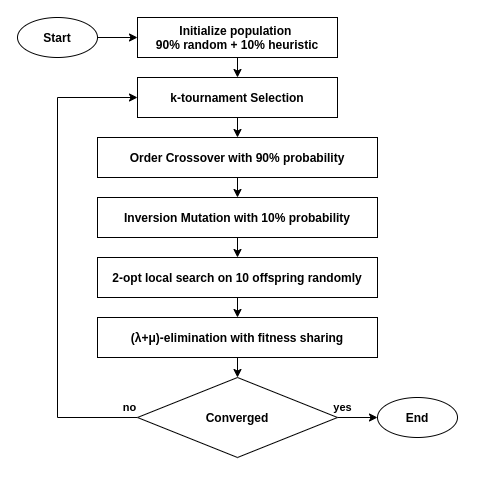
\includegraphics[width=0.5\textwidth]{images/genetic_algorthm_main_loop.png}
\caption{A high level flowchart of the developed evolutionary algorithm.}
\label{fig:main_loop}
\end{figure}

Selection is done with replacement, so that there is increased probability to pick really good individuals multiple times to recombine with other individuals. We basically desire good genes to be reused in the next generation.

A $(\lambda+\mu)-elimination$ operator selects the new population by combining the old population with the new offspring, sorting the combined population and keeping the $top-\lambda$ individuals. Because of the fitness sharing scheme that is used, the elimination method selects individuals sequentially and not in parallel, with replacement. After each selection the combined population plus offspring are reweighted, so as to avoid several similar solutions from surviving to the next generation.

\subsection{Parameter selection}\label{ss:parameter_selection}

%\ReplaceMe{For all of the parameters that are not automatically determined by adaptivity or self-adaptivity (as you have described above), describe how you determined them. Did you perform a hyperparameter search? How did you do this? How did you determine these parameters would be valid both for small and large problem instances?}

Because of the addition of local search and fitness sharing, the algorithm grew more computationally expensive. As a result the population size and the offspring size were significantly reduced by two orders of magnitude to allow the algorithm to run for more generations before time runs out. In particular, $\lambda$ was reduced from $2000$ to $10$ and $\mu$ was reduced from around $2000/3$ to $10$. These parameters were tuned to achieve good performance in all problems, big and small. Figure \ref{fig:lambda_search} presents the performance of the algorithm on $tour194$ for $\lambda$ values between $10$ and $100$ and $\mu$ values defined as $\mu = \lambda$. The reduction of the population $\lambda$ and offspring size $\mu$ means that the algorithm can produce more generation before time runs out.

For mutation, the idea of mass mutation from Eiben et al \cite{eiben} was applied. This mass mutation approach refers mostly to memetic algorithms, which find really good locally optimal solutions using local search operators. The goal of mass mutation is to apply mutation with a really high rate so that the algorithm can find solutions that escape from local minima. This approach is implemented with a mutation probability $p_m = 0.9$. Figure \ref{fig:pm_search} presents the best fitness for various mutation rates from 0.1 to 1.0 on $tour194$.

The number $k$ of participants in the tournament selection was chosen via hyperparameters search. The results are shown in Figure \ref{fig:k_search}, where a $k=4$ was chosen due to its nice balance between performance and computational load.

The fitness sharing parameters $\alpha$ and $\sigma$ were selected as 1 and $num\_cities / 5$ ($38$ for $tour194$) respectively, balancing performance and diversity. The shape parameter $\alpha$ is average with regard to punishment of similar candidates, while the distance $\sigma$ is selected with respect to the size of the problem. It wouldn't be prudent to select the same distance threshold for all problem sizes, since a threshold of $\sigma=5$ might be suitable for the smallest $tour29$ problem, but it would result in a very homogeneous population for the largest problem $tour929$. Figure \ref{fig:sigma_search} presents the best fitness for various $\sigma$ values in range of one tenth of the number of cities $N$ to $N$ on $tour194$.

All of the aforementioned parameters were tested with regard to whether they allowed the algorithm to run for enough generations on each problem and whether they produced good enough solutions. The full list of selected hyperparameters can be seen in Subsection \ref{ss:metadata}.

\begin{figure}[H]
\centering
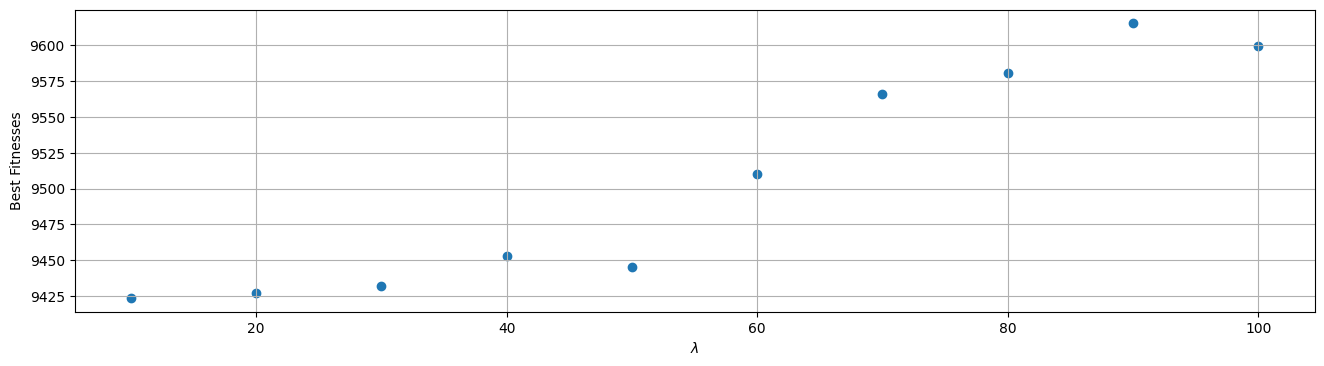
\includegraphics[width=\textwidth]{results/tuning/lambda_hyperparameter_search.png}
\caption{Hyperparameter search of $\lambda$}\label{fig:lambda_search}
\end{figure}%

\begin{figure}[H]
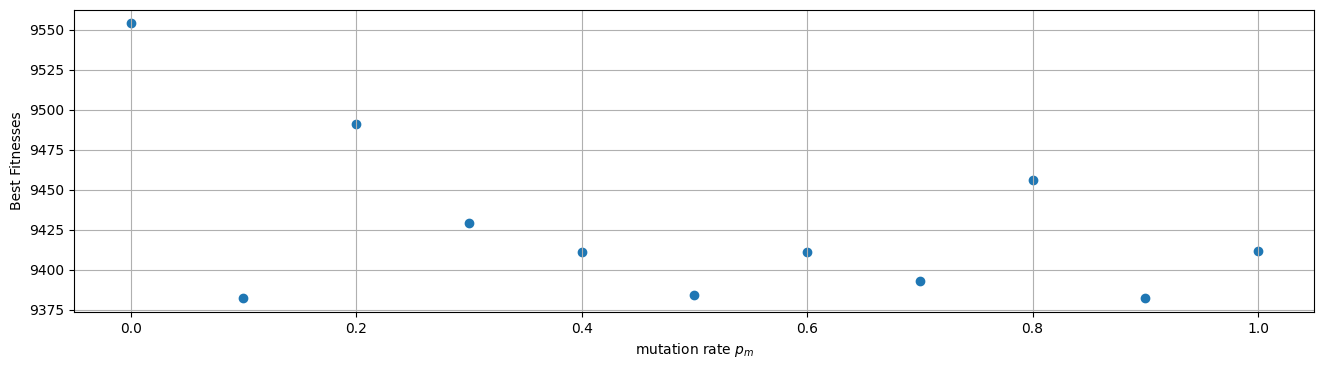
\includegraphics[width=\textwidth]{results/tuning/mutation_rate_hyperparameter_search.png}
\caption{Hyperparameter search of mutation rate $p_m$}
\label{fig:pm_search}
\end{figure}%

\begin{figure}[H]
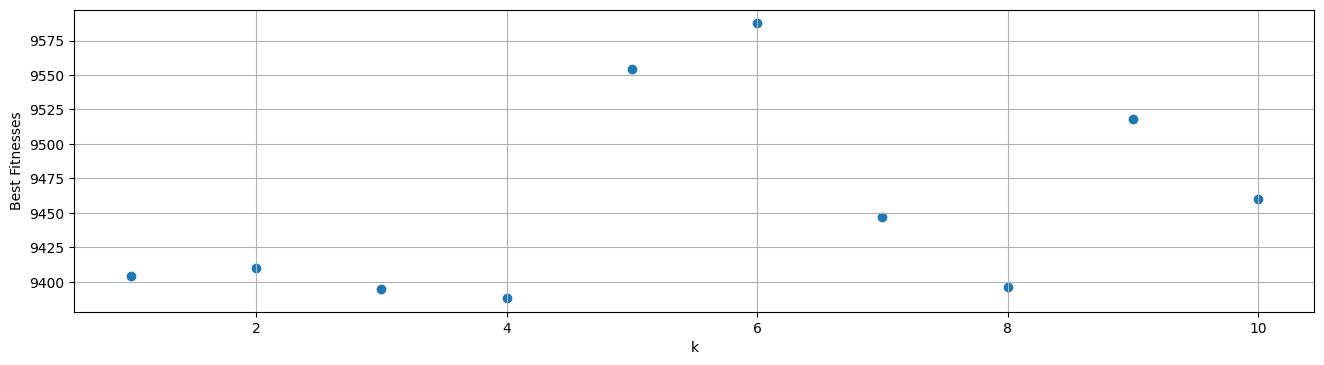
\includegraphics[width=\textwidth]{results/tuning/k_hyperparamter_search.png}
\caption{Hyperparameter search of $k$ in $k$-tournament selection}
\label{fig:k_search}
\end{figure}%

\begin{figure}[H]
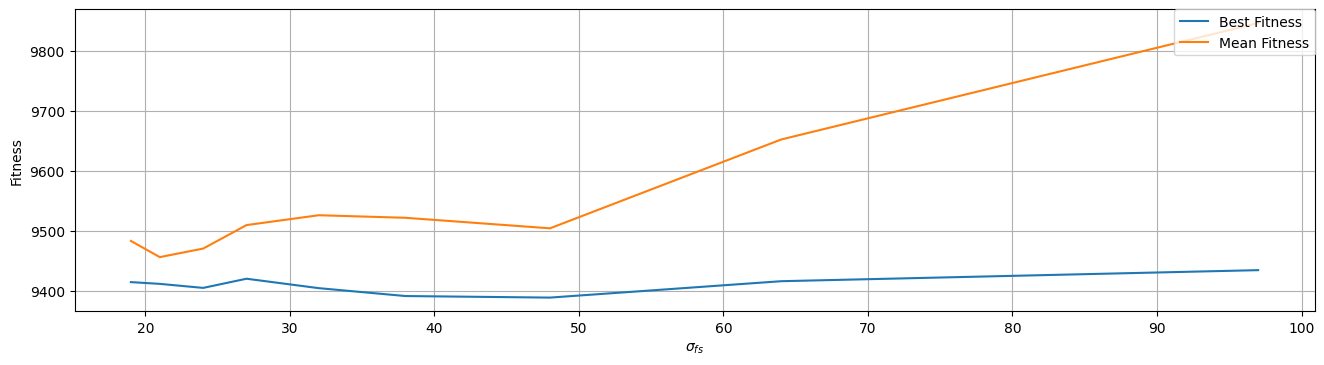
\includegraphics[width=\textwidth]{results/tuning/fs_sigma_hyperparamter_search.png}
\caption{Hyperparameter search of fitness sharing $\sigma$ for $\sigma=num\_cities/d$, where $d \epsilon \{1,2,3,4,5,6,7,8,9,10\}$}
\label{fig:sigma_search}
\end{figure}%

%Another parameter that was added in the individual phase is the mutation strength $\sigma_m$, which was also tuned via hyperparameter search. The results are shown in Figure \ref{fig:sigma-mu}. The algorithm achieved the best results for $\sigma_m = 3$, although, it could just be a matter of luck. A more thorough hyperparameter search would repeatedly run the same experiment and then decide the best value based on the average of the results.

%\begin{figure}[H]
%    \centering
%	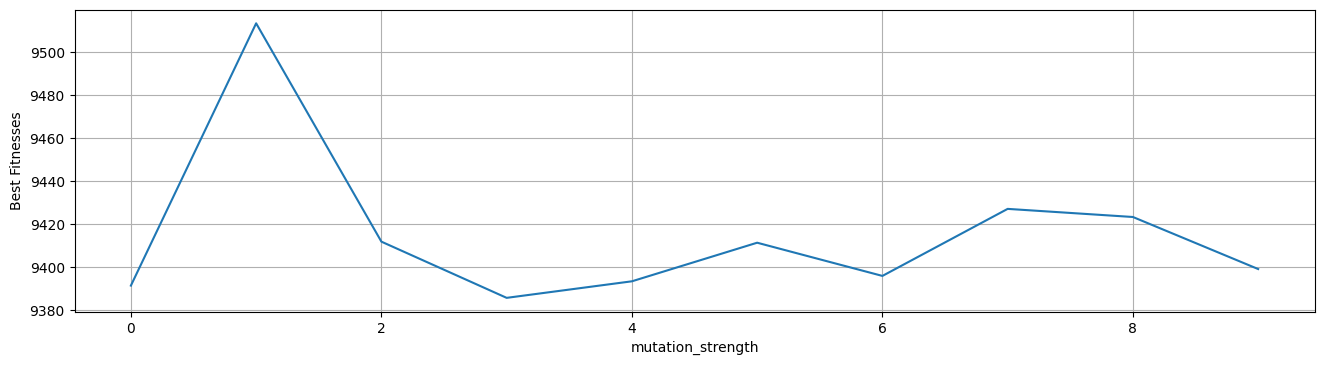
\includegraphics[width=\textwidth]{results/tuning/sigma_mu.png}
%    \caption{Best Fitness for various mutation strength values. Experiment was run on \textit{tour194}}
%    \label{fig:sigma-mu}
%\end{figure}

%\subsection{Other considerations}

%\ReplaceMe{Did you consider other items not listed above, such as elitism, multiobjective optimization strategies (e.g., island model, pareto front approximation), a parallel implementation, or other interesting computational optimizations (e.g. using advanced algorithms or data structures)? You can describe them here or add additional subsections as needed.}


\section{Numerical experiments} \label{s:numerical_experiments}

%\RemoveMe{\textbf{Goal:} Based on this section and our execution of your code, we will evaluate the performance (time, quality of solutions) of your implementation and your ability to interpret and explain the results on benchmark problems.}

\subsection{Metadata} \label{ss:metadata}

%\ReplaceMe{What parameters are there to choose in your evolutionary algorithm? Which fixed parameter values did you use for all experiments below? If some parameters are determined based on information from the problem instance (e.g., number of cities), also report their specific values for the problems below.

%Report the main characteristics of the computer system on which you ran your evolutionary algorithm. Include the processor or CPU (including the number of cores and clock speed), the amount of main memory, and the version of Python 3.}

The following list presents the different parameters that were chosen for the experiments presented in the following subsections. 
\begin{itemize}
\item $\lambda = 10$: size of population
\item $\mu = 10$: size of offspring
\item $\lambda_h = 0.2 \times \lambda = 2$: number of heuristic solutions calculated during initialization
\item $k = 4$: number of individuals in the k-tournament selection
\item $p_c = 0.9$: recombination probability per generation
\item $p_m = 0.9$: mutation probability per generation
\item $p_l = 1.0$: local search probabiility per generation
\item $\sigma_m = 1$: mutation strength
\item $\alpha_{fs} = 1$: Fitness sharing shape
\item $\sigma_{fs} = \frac{N}{5}$: Fitness sharing distance threshold, where N is the size of the problem (eg. for $tour29$ $N=29$)
\end{itemize}

All experiments were run in a laptop with an Intel i7 processor with 4 physical cores, 8 logical cores, 8GB Ram, and a clock speed of 1.3GHz (3.9GHz turbo speed). No parallelization was used, so execution was limited to one core. Finally, all experiments were run with \textit{Python 3.8.5}.

\subsection{tour29.csv} \label{ss:tour29}

%\ReplaceMe{Run your algorithm on this benchmark problem (with the 5 minute time limit from the Reporter). Include a typical convergence graph, by plotting the mean and best objective values in function of the time (for example based on the output of the Reporter class). 

%What is the best tour length you found? What is the corresponding sequence of cities? 

%Interpret your results. How do you rate the performance of your algorithm (time, memory, speed of convergence, diversity of population, quality of the best solution, etc)? Is your solution close to the optimal one?

%Solve this problem 1000 times and record the results. Make a histogram of the final mean fitnessess and the final best fitnesses of the 1000 runs. Comment on this figure: is there a lot of variability in the results, what are the means and the standard deviations?}

Figure \ref{fig:tour29convergence} presents a typical convergence graph of the algorithm run on \textit{tour29}. The algorithm finds the optimal value in about 3 seconds and converges after 200 generations of no improvement in about 7 seconds. Furthermore, the mean fitness never converges fully to the best fitness because of the fitness sharing scheme that is used, which indicates good preservation of diversity across generations.

\begin{figure}
\begin{subfigure}[t]{0.5\textwidth}
    \centering
	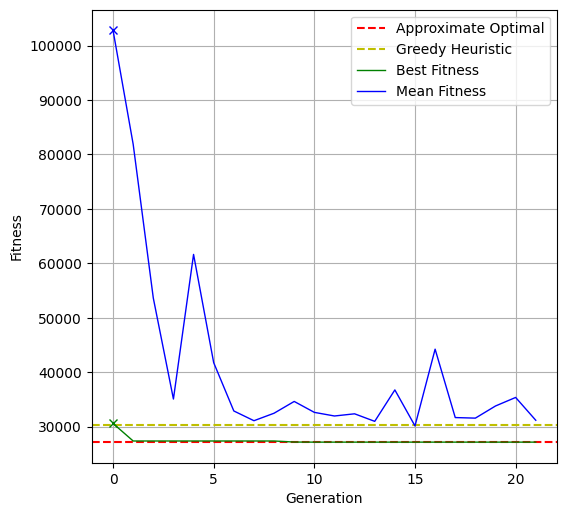
\includegraphics[width=\textwidth]{results/4.2/tour29_convergence.png}
    \caption{Tour29}
    \label{fig:tour29convergence}
\end{subfigure}
\begin{subfigure}[t]{0.5\textwidth}
    \centering
	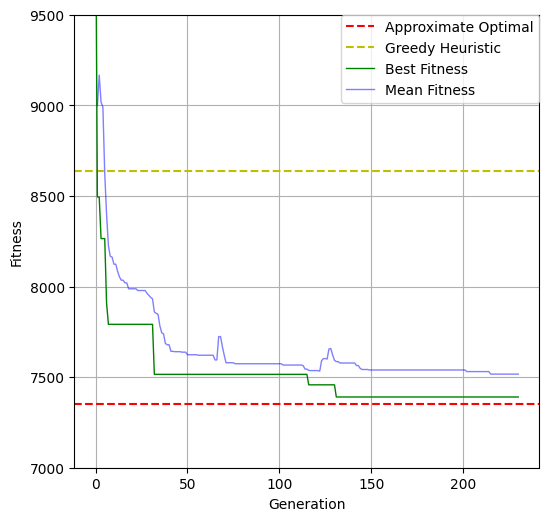
\includegraphics[width=\textwidth]{results/4.3/tour100_convergence.png}
    \caption{Tour100}
    \label{fig:tour100convergence}
\end{subfigure}\\
\begin{subfigure}[t]{0.5\textwidth}
    \centering
	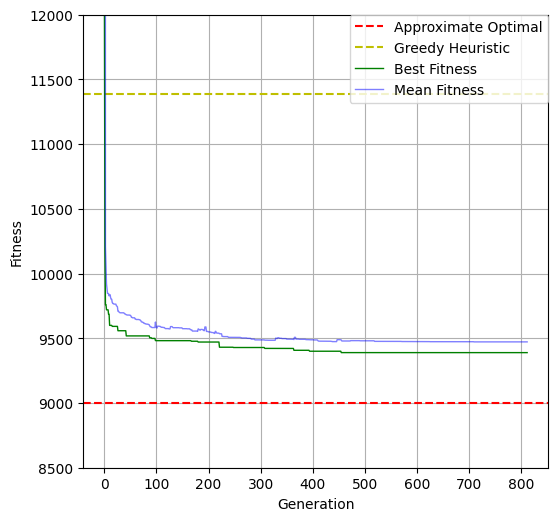
\includegraphics[width=\textwidth]{results/4.4/tour194_convergence.png}
    \caption{Tour194}
    \label{fig:tour194convergence}
\end{subfigure}
\begin{subfigure}[t]{0.5\textwidth}
    \centering
	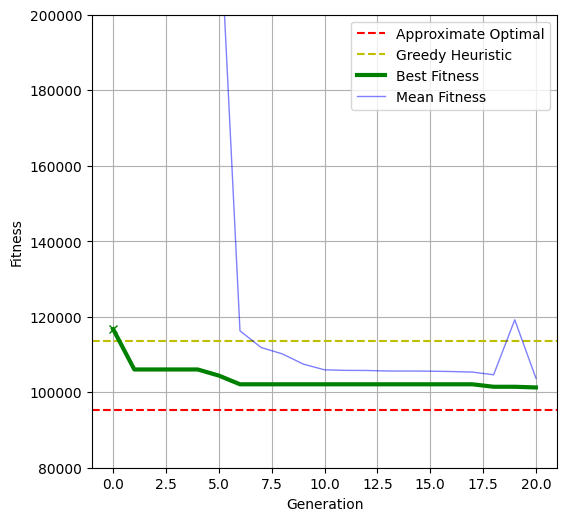
\includegraphics[width=\textwidth]{results/4.5/tour929_convergence.png}
    \caption{Tour929}
    \label{fig:tour929convergence}
\end{subfigure}
\caption{Typical convergence graphs on the various datasets.}
\end{figure}

The best tour that was found has a fitness - tour length of approximately $\textbf{27154.48839924464m}$. The corresponding tour sequence is the following:
\begin{center}
\textit{[6, 8, 12, 13, 15, 23, 24, 26, 19, 25, 27, 28, 22, 21, 20, 16, 17, 18, 14, 11, 10, 9, 5, 0, 1, 4, 7, 3, 2]}
\end{center}

\begin{figure}[H]
     \centering
     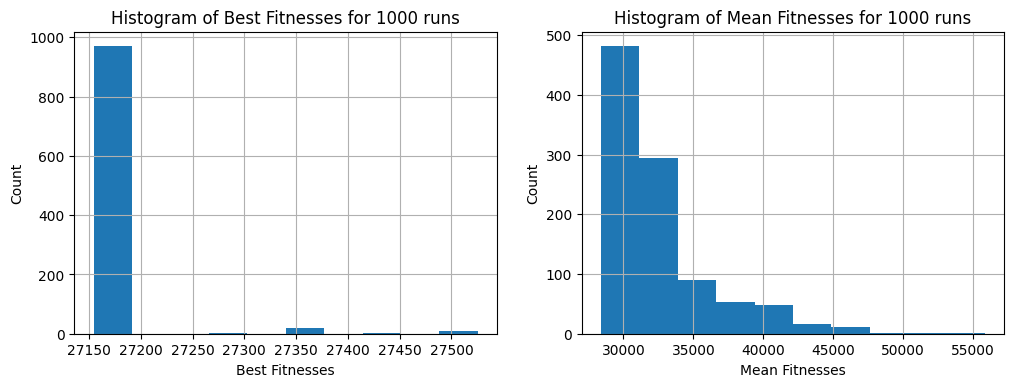
\includegraphics[width=\textwidth]{results/4.2/tour29_histogram.png}
     \caption{Tour29 1000 run histograms of best and mean fitness}
     \label{fig:tour29histogram}
\end{figure}

Based on Figure \ref{fig:tour29histogram}, the algorithm seems to perform really well on \textit{tour29}, consistently finding the optimal or a near optimal solution for a $1000$ runs. At the same time, the histogram of the mean fitness illustrates the fact that even at convergence the algorithm manages to preserve some diversity in the population, since mean fitness is always greater than the best fitness. The mean and std of the 1000 runs for the best and the mean fitness are shown in Table \ref{table:1000run_statistics}.

\begin{table}[H]
\centering
\begin{tabular}{ |c|c|c|c| } 
\hline
Fitness & 1000-Run Average & 1000-Run Sandard Deviation\\
\hline
Best & $27160.06137471839$ & $43.44519234412967$ \\ 
Mean & $27497.005460551067$ & $92.03286853386737$ \\ 
\hline
\end{tabular}
\caption{Statistics of 1000 runs on \textit{tour29}.}
\label{table:1000run_statistics}
\end{table}


\subsection{tour100.csv} \label{ss:tour100}

%\ReplaceMe{Run your algorithm on this benchmark problem (with the 5 minute time limit from the Reporter). Include a typical convergence graph, by plotting the mean and best objective values in function of the time (for example based on the output of the Reporter class). 
%
%What is the best tour length you found in each case? 
%
%Interpret your results. How do you rate the performance of your algorithm (time, memory, speed of convergence, diversity of population, quality of the best solution, etc)? Is your solution close to the optimal one?}

Figure \ref{fig:tour100convergence} presents the fitness and mean fitness of a run of the algorithm on \textit{tour100}. The algorithm converged on the 346th generation taking 77 seconds and the best solution that was found comes very close to the optimal solution (red dotted line). Although, this solution was found before generation \#150, it took 200 more generations until convergence. The diversity promotion scheme performed really well as can be seen from the distance between the mean and best fitness across generations.

The best tour that was found has a fitness - tour length of approximately $\textbf{7401.970200443819m}$. The corresponding tour sequence is the following:\\

\begin{minipage}{\textwidth}
\centering
\textit{[92, 52, 60, 2, 47, 35, 25, 71, 55, 80, 16, 20, 63, 24, 97, 98, 48, 40, 44, 78, 33, 90, 85, 70, 27, 22, 77, 96, 69, 29, 1, 17, 34, 95, 76, 68, 23, 49, 18, 59, 5, 56, 57, 19, 73, 39, 32, 74, 38, 13, 8, 86, 4, 51, 54, 41, 12, 89, 61, 43, 58, 67, 42, 83, 66, 0, 50, 65, 15, 79, 64, 93, 14, 6, 88, 72, 94, 84, 36, 46, 91, 28, 10, 37, 45, 7, 62, 53, 11, 87, 30, 9, 3, 31, 82, 21, 75, 99, 26, 81]}
\end{minipage}

\subsection{tour194.csv} \label{ss:tour194}

%\ReplaceMe{Run your algorithm on this benchmark problem (with the 5 minute time limit from the Reporter). Include a typical convergence graph, by plotting the mean and best objective values in function of the time (for example based on the output of the Reporter class). 
%
%What is the best tour length you found? 
%
%Interpret your results. How do you rate the performance of your algorithm (time, memory, speed of convergence, diversity of population, quality of the best solution, etc)? Is your solution close to the optimal one?}

Figure \ref{fig:tour194convergence} presents the fitness and mean fitness of a run of the algorithm on \textit{tour194}. The best solution that was found lies between the greedy heuristic (yellow dotted line) and the optimal one (red dotted line). It is closer to the optimal one and a clear improvement rate can be observed across iterations. The algorithm finds the best solution at about the 320th iteration, but it doesn't converge until the timeout at around the 570th generation, since there haven't been over 200 iterations without improvement. Furthermore, the diversity promotion scheme managed to keep enough diversity which can be observed by the nonzero distance between the best and mean fitnesses.

The best tour that was found has a fitness - tour length of $\textbf{9385.50274991716m}$. The algorithm converged on the 812th generation taking 177 seconds. The corresponding tour sequence is the following:

\begin{center}
\textit{[46, 50, 60, 66, 72, 65, 67, 63, 69, 76, 83, 80, 78, 82, 87, 91, 96, 94, 95, 92, 90, 101, 102, 105, 104, 106, 107, 99, 109, 111, 114, 115, 116, 120, 119, 122, 123, 127, 132, 128, 134, 142, 147, 159, 165, 170, 169, 166, 161, 157, 158, 164, 167, 177, 179, 184, 192, 187, 190, 191, 188, 183, 180, 176, 174, 172, 173, 171, 178, 185, 182, 186, 189, 193, 181, 175, 168, 163, 162, 160, 155, 129, 126, 124, 125, 131, 133, 136, 139, 144, 148, 145, 141, 137, 138, 143, 149, 153, 156, 152, 151, 140, 146, 150, 154, 135, 130, 117, 121, 118, 108, 112, 113, 110, 103, 100, 98, 93, 88, 89, 97, 84, 85, 64, 19, 62, 35, 58, 61, 81, 70, 79, 86, 75, 74, 77, 71, 73, 68, 59, 56, 44, 36, 26, 21, 28, 27, 32, 17, 20, 23, 25, 16, 6, 10, 13, 24, 22, 12, 15, 7, 5, 0, 3, 1, 2, 4, 8, 9, 11, 14, 18, 29, 31, 30, 34, 37, 40, 47, 45, 43, 41, 49, 48, 54, 53, 51, 52, 55, 57, 42, 39, 33, 38]}
\end{center}

\subsection{tour929.csv} \label{ss:tour929}

%\ReplaceMe{Run your algorithm on this benchmark problem (with the 5 minute time limit from the Reporter). Include a typical convergence graph, by plotting the mean and best objective values in function of the time (for example based on the output of the Reporter class). 
%
%What is the best tour length you found? 
%
%Interpret your results. How do you rate the performance of your algorithm (time, memory, speed of convergence, diversity of population, quality of the best solution, etc)? Is your solution close to the optimal one? 
%
%Did your algorithm converge before the time limit? How many iterations did you perform?}

Figure \ref{fig:tour929convergence} presents the fitness and mean fitness of a run of the algorithm on \textit{tour929}. The best solution that was found is significantly better than the greedy heuristic (yellow dotted line) and fairly close to the optimal one (red dotted line). The algorithm didn't converge before the timeout after the 228th generation. Furthermore, the diversity promotion scheme managed to keep enough diversity which can be observed by the nonzero distance between the best and mean fitnesses.


The best tour that was found has a fitness - tour length of approximately $\textbf{96953.57508056797m}$. The corresponding tour sequence is the following:
\begin{center}
\textit{[925, 927, 922, 920, 918, 913, 907, 894, 899, 916, 917, 915, 912, 910, 909, 911, 906, 904, 903, 898, 893, 890, 897, 887, 884, 863, 853, 843, 830, 804, 826, 834, 835, 854, 857, 861, 870, 881, 871, 873, 877, 878, 883, 872, 865, 864, 851, 846, 847, 859, 845, 841, 827, 832, 818, 811, 627, 628, 645, 723, 765, 783, 787, 813, 814, 812, 802, 803, 788, 792, 790, 807, 815, 805, 806, 808, 809, 797, 774, 768, 776, 770, 757, 758, 752, 748, 756, 762, 767, 760, 771, 784, 775, 786, 791, 798, 801, 799, 800, 785, 782, 789, 780, 769, 750, 749, 739, 731, 727, 712, 703, 698, 696, 688, 689, 701, 711, 718, 724, 734, 737, 728, 715, 699, 694, 684, 697, 713, 740, 753, 766, 747, 742, 702, 683, 658, 642, 668, 677, 670, 666, 674, 657, 656, 659, 669, 673, 676, 681, 693, 680, 678, 671, 652, 651, 654, 667, 655, 644, 639, 643, 650, 653, 660, 665, 695, 709, 710, 720, 733, 735, 746, 751, 755, 764, 773, 778, 781, 772, 761, 763, 716, 706, 708, 719, 736, 741, 738, 730, 717, 705, 714, 722, 732, 721, 704, 707, 700, 692, 690, 691, 682, 675, 664, 679, 672, 641, 640, 610, 528, 609, 595, 586, 580, 572, 579, 590, 603, 608, 607, 598, 589, 585, 577, 569, 568, 556, 547, 540, 557, 541, 532, 527, 518, 506, 499, 498, 480, 471, 463, 455, 448, 441, 454, 462, 492, 505, 526, 531, 536, 546, 555, 571, 576, 584, 593, 594, 602, 606, 611, 619, 620, 615, 633, 635, 634, 663, 686, 794, 777, 726, 662, 685, 743, 661, 810, 793, 725, 624, 623, 614, 622, 618, 617, 599, 581, 582, 604, 600, 605, 601, 583, 567, 566, 561, 554, 560, 553, 552, 539, 530, 524, 523, 510, 509, 522, 515, 521, 534, 543, 537, 544, 538, 535, 545, 551, 565, 564, 563, 559, 550, 508, 438, 443, 433, 426, 439, 434, 445, 444, 451, 466, 473, 467, 474, 484, 495, 496, 511, 516, 512, 502, 486, 476, 485, 475, 456, 452, 446, 457, 468, 447, 453, 477, 469, 487, 513, 488, 478, 458, 479, 490, 489, 497, 517, 525, 503, 504, 491, 461, 470, 460, 459, 440, 435, 428, 427, 418, 417, 406, 400, 401, 413, 402, 407, 420, 421, 429, 422, 430, 431, 423, 416, 408, 409, 410, 419, 399, 395, 389, 387, 376, 378, 388, 386, 382, 394, 396, 398, 405, 404, 415, 414, 403, 393, 392, 391, 384, 385, 381, 377, 355, 357, 348, 345, 346, 343, 333, 352, 375, 341, 342, 339, 344, 340, 331, 337, 363, 373, 370, 366, 367, 379, 432, 449, 450, 493, 500, 573, 587, 596, 562, 464, 397, 360, 368, 371, 380, 390, 411, 436, 442, 481, 482, 472, 501, 570, 613, 574, 592, 591, 629, 795, 729, 838, 817, 823, 844, 858, 868, 875, 852, 848, 839, 820, 646, 630, 636, 687, 616, 632, 558, 514, 437, 424, 412, 356, 361, 353, 351, 350, 329, 325, 315, 309, 303, 304, 297, 306, 293, 273, 272, 256, 265, 264, 260, 269, 271, 281, 285, 270, 314, 318, 284, 274, 313, 292, 283, 259, 253, 250, 268, 282, 327, 326, 324, 244, 305, 296, 254, 236, 92, 93, 87, 83, 84, 85, 81, 45, 48, 80, 77, 89, 200, 99, 62, 39, 41, 40, 21, 7, 1, 5, 43, 31, 24, 23, 25, 22, 11, 16, 8, 6, 0, 18, 26, 51, 67, 65, 78, 131, 132, 102, 96, 88, 72, 59, 36, 32, 27, 12, 14, 9, 2, 3, 4, 10, 17, 13, 30, 29, 19, 28, 35, 33, 20, 38, 37, 46, 44, 50, 52, 53, 55, 54, 60, 63, 66, 70, 69, 74, 68, 73, 82, 86, 95, 98, 229, 251, 261, 288, 298, 299, 302, 294, 310, 316, 320, 334, 323, 301, 300, 290, 286, 289, 278, 266, 243, 248, 245, 249, 252, 255, 257, 267, 262, 276, 263, 258, 204, 153, 237, 203, 180, 165, 161, 147, 143, 130, 109, 105, 108, 104, 120, 124, 126, 133, 145, 156, 146, 154, 159, 174, 182, 185, 187, 199, 214, 227, 233, 222, 211, 208, 206, 193, 190, 186, 176, 173, 179, 172, 181, 184, 192, 205, 202, 194, 189, 196, 207, 215, 217, 221, 225, 234, 228, 216, 226, 235, 239, 240, 242, 246, 247, 241, 238, 232, 230, 224, 223, 210, 198, 213, 201, 188, 177, 175, 169, 167, 163, 160, 148, 141, 139, 137, 144, 151, 171, 168, 162, 157, 155, 140, 128, 138, 164, 166, 183, 195, 209, 197, 212, 218, 220, 231, 219, 191, 170, 150, 106, 112, 111, 121, 107, 116, 129, 113, 103, 114, 119, 123, 136, 134, 135, 142, 149, 158, 152, 125, 127, 122, 118, 117, 115, 110, 100, 91, 58, 61, 101, 97, 90, 94, 75, 42, 47, 56, 57, 49, 15, 34, 64, 71, 76, 79, 178, 287, 308, 307, 330, 332, 338, 347, 359, 362, 354, 358, 365, 383, 520, 533, 597, 519, 507, 549, 588, 626, 575, 621, 649, 631, 625, 548, 483, 425, 372, 335, 336, 322, 321, 291, 312, 275, 277, 280, 279, 295, 311, 319, 317, 328, 349, 374, 364, 369, 465, 494, 529, 542, 578, 612, 637, 647, 648, 754, 816, 744, 638, 759, 796, 825, 833, 855, 849, 856, 866, 869, 888, 891, 892, 889, 885, 874, 880, 879, 886, 882, 876, 862, 842, 837, 836, 831, 828, 824, 779, 745, 822, 821, 819, 829, 840, 850, 860, 867, 895, 902, 896, 900, 901, 905, 908, 914, 919, 928, 926, 923, 921, 924]}
\end{center}

\section{Critical reflection} \label{s:critical_reflection}

%\RemoveMe{\textbf{Goal:} Based on this section, we will evaluate your understanding and insight into the main strengths and weaknesses of your evolutionary algorithms.}

%\ReplaceMe{Describe the main lessons learned from this project. What do you think are the main strong points of evolutionary algorithms in general? Did you apply these strengths in this project? What are the main weaknesses of evolutionary algorithms and of your implementation in particular? Do you think these can be avoided or mitigated? How? Do you believe evolutionary algorithms are appropriate for this problem? Why (not)? What surprised you and why? What did you learn from this project?}

Working on this project allowed me the opportunity me to study evolutionary algorithms and understand them in more depth, while also looking at state-of-the-art research to find clues as to how to refine my algorithm for solving the \textit{Travelling Salesman Problem (TSP)}. Evolutionary algorithms in general are really good at solving non-convex optimization problems whose solution space contains many local minima, where a popular optimization algorithm like Steepest Descent would get stuck quite easily in a suboptimal solution. TSP is such a non-convex problem and hence evolutionary algorithms are a good approach to solve it. Of course in most cases it's not guaranteed that an evolutionary algorithm will find the global optimum in finite time, but it certainly has the capability to escape local minima and find really good solutions. This is mainly thanks to the random nature of the mutation and recombination steps. On one hand we have the random combination of the useful information that already exists in the population and on the other hand we have the randomness that's inserted into new individuals, which may produce even better solutions than the previous generations.

A good evolutionary algorithm, in general, needs really careful design and needs to be specialized to a problem and use problem specific information to guide the search towards optimal solutions. For example, it's easy to design an evolutionary algorithm for solving the TSP with a lot of randomness, but to make it really efficient, it is very advantageous to seed the initial population or even other steps of the algorithm with heuristic information. This step proved to improve the efficiency of the developed algorithm and speed up the search of good candidate solutions quite considerably. Moreover, an evolutionary algorithm can become even more efficient if it's combined with local search methods like steepest descent or k-opt. Instead of waiting to find local minima after many generations of mutation and recombination it's a lot more efficient to run local search on a lot of individuals from the population and thus find many local minima, thus increasing the probability to find the global minima or at least a really good solution. The introduction of 2-opt proved instrumental in finding really good solutions without letting the algorithm run for thousands of generations.

Of course, evolutionary algorithms are not the perfect tool for solving any problem in many cases there are way better alternatives. One main disadvantage of evolutionary algorithms is that they are very computationally expensive. The developed evolutionary algorithm, in particular, is quite inefficient because of the really expensive local search operator (2-opt) that prevents the larger problems from running for a high number generations given the 5-minute time limit. This could have potentially been alleviated by parallelizing the local search on multiple offspring at the same time. Another issue with the local search operator and the greedy heuristic initialization was that the algorithm was directed towards strong local minima and couldn't escape easily. However, the benefit of those two methods far outweighed the costs.

What surprised me the most in this project was mainly how modular and customizable an evolutionary algorithm can be. There are so many different methods to choose from, yet not all of them are compatible with all problems or with each other and it's a quite complex and time-consuming task to find the right ones to combine. Furthermore, a few methods that I experimented with, such as self-adaptive mutation rate and/or strength failed to provide any measurable improvement to the algorithm, despite them being quite popular in the literature. Another thing that was quite difficult to work out was how to interpret the results. Due to the random nature of evolutionary algorithms, it was difficult for example to evaluate if a modification to the algorithm or the tuning of a parameter made any difference, which resulted in a lot of trial and error to find a good combination of parameters.

%\section{Other comments} \label2{sec_other}
%
%\ReplaceMe{In case you think there is something important to discuss that is not covered by the previous sections, you can do it here. }

\bibliographystyle{plain}
\bibliography{ref}

\end{document}
